% !Mode:: "TeX:UTF-8"

\chapter{模型设定}{Model Specification}
\label{chap03}

本章主要介绍模型的构建,将试图建立一个由人口因素驱动的\dns{},通过考察\ds 的动态特征,论证其反映的货币市场长期均衡时的利率水平的变动状况,即\dsf 决定了动态~Nelson-Siegel~ 模型中的长期影响因子。同时,该部分将对本文所使用的数据进行相应的说明。

\section{模型}
记~$y_t(\tau)$~为一个剩余到期期限为~$\tau$~期的债券到期收益率,该变量可以分解为两部分:(1)一个由经济系统中的永久性冲击决定的长期均衡利率水平的组成部分,记为~$K_t(\tau)$,该状态随\dsf 在周期长度为一个世代交叠的频度上变化;(2)一个反映商业周期冲击的局部均值回复的组成部分,$X_t(\tau)$:
\begin{align}\label{chap03:yield}
   y_t(\tau) & = K_t(\tau) + X_t(\tau),
 \end{align}
式中~$K_t$~代表了利率中受到经济永久性冲击的长期项(预期水平),而~$X_t$~ 是利率中的代表条件均值为~0~的均值回复项。
在\cneqref{chap03:yield}中,长期项~$K_t$~对应于\cneqref{dns}中表示\dns 的水平因子(Level Factor),受到经济系统基础层面的影响,如代表性消费者的投资风险厌恶程度的改变、社会结构尤其是人口年龄结构的波动等。而反映短期利率变化的均值回复项~$X_t$~对应于\dns 的斜度因子(Slope Factor)与曲度因子(Curvature Factor)。

\subsection{人口年龄结构与长期利率水平}
在第(\ref{theory&model})章有关\ts 的理论与模型的讨论中,利率在较长期限内表现为均值回复(Mean-Reverting)的特性,以往的模型缺少对这一方面做深入的经济解释,特别是推动长期利率水平的波动的基础因素(fundamental factors)。现代时间序列理论表明,模型变量的可预测性主要有该数据时间序列中具有的趋向均值性质的长期影响因子所决定。

根据利率期限结构的期望理论(Expectation Hypothesis of the Term Structure),一个~$\tau$~期的利率由该时期内短期利率的数算平均值加上一个期限贴水(term premium),这意味着对于一个~$\tau$~期的无风险利率可以表示为该时期内单期无风险即期利率的算术平均值,即利率的长期期望值为:
  \begin{align}\label{k}
   K_{t}(\tau) &=  \frac{1}{\tau}\sum_{j=0}^{\tau-1}K_{t+j|t},
 \end{align}
 式中~$K_{t+j|t}$~表示在当前时期~$t$~对未来~$t+j$~期的即期利率的预测,即~$K_{t+j|t}=\E_t[K_{t+j}|\mathcal{I}_t]$,
 其中~$\mathcal{I}_t=\{\mathcal{I}_{t-1},\mathcal{I}_{t-2},\ldots\}$~ 为市场上已知的所有信息集。

\cneqref{chap03:yield} 表明即期利率并非一个平稳的时间序列,而是一个趋向于时变水平的非平稳序列。\citeai{fama1987information}指出利用不同期限的远期利率有效可以提高对未来即期利率的预测,并推断这是由于即期利率朝向一个不变的预期利率水平回复的特征决定的。而\citeai{fama2006behavior}利用美国国债券~1986~年到~2004~年的数据对该模型做了重新检验,发现现有的数据并不支持预期的均值回复利率水平是一个固定数值的说法,而是趋向一个时变的长期利率水平,这个长期的利率水平受到经济系统中永久性冲击(permanent shocks)的影响,从而在时间序列上表现为水平的波动。相类似的,\citeai{balduzzi1998central} 认为,即期利率既有一个向条件均值(conditional mean)靠拢的特性,长期债券收益率包含有对短期利率预测的信息,同时,即期利率中还含有一个时变的中央趋势(central tendency),即利率趋向一个长期限债券收益率的特性。因此,为了更好地对利率的未来波动进行预测,必须建立一个包含代表条件均值的短期债券收益与一个代表中央趋势的长期债券收益的因子模型才能提高对利率的预测能力。而远期利率对未来即期利率的预测能力主要归功于利率中所包含的具有平稳特性的趋势组成部分,这一组成部分本身与随着时间而变动,并非一个固定的数值。对于如何建立即期利率的预测模型,问题的关键在于正确刻画即期利率中能够代表长期持久性变动方向的驱动因素。

 然而,对于经济系统中的何种冲击能够被视为永久性冲击可以对利率产生影响,目前的研究成果并不足以令人信服。比如,由~Fisher~方程
\begin{align}
  r_t &= i_t - \pi_{t+1}^e,
\end{align}
可知实际利率为名义利率与预期通货膨胀率的函数关系,则可以通过该关系来解释利率的变动。例如\citeai{goto2003conquest}认为美联储在货币供给政策上的转变导致预期通货膨胀率的变化,这种机制转变(regime shift)是导致利率水平波动的主要原因。然而,这种解释依然没有抓住决定问题的关键:即使是美联储的行为也是一种内生性的反映,同其他内生变量一样受到经济系统各种变量的外生冲击。因此,需要进一步探讨影响利率的长期动态行为特征的结构性变化。本文认为,这个反映长期利率变动方向的水平因素(Level Factor)受到经济系统基础层面的影响,如代表性消费者的投资风险厌恶程度的改变、社会结构尤其是人口年龄结构的波动等。\ds 作为一个重要的影响因素与\ts 的长期均衡水平的波动存在着密切的关系。这类由\ds 的变动所引致的对\tsm 的影响只有在一个世代期限范畴内才能显现效果。

在\cneqref{k}中,进一步假设这个未来的即期利率由社会人口的年龄结构分布决定。或者换一个角度看,如\citeai{favero2012demographics}认为各国的中央银行在做货币政策决策时,都会考虑到社会的人口结构特征对政策传导机制的影响。因此,即期利率可以由表示人口年龄结构变化的变量~$MY_t$~来表示:
 \begin{align}
   K_{t+j|t}  &= \omega_t MY_{t+j|t}+\eps_t, \quad \eps_t \sim \mathcal{N}(0,\sigma^2_{\eps})\\
   MY_{t+j|t} &= \E_t [MY_{t+j}|\mathcal{I}_t],\quad \mathcal{I}_t=\{\mathcal{I}_{t-1},\mathcal{I}_{t-2},\ldots\}
 \end{align}
式中$MY_{t+j|t}$~是金融市场对未来人口年龄结构变化的预测,该预测值可以在美国人口调查局(Bureau of the Census,BoC)提供的人口预测项目中查到,具有一定的可信度。模型参数~$\omega_t$~表示被预测到的\dsf 对当期即期利率的影响因子。

因此,未来~$\tau$~期的长期利率水平可以表示为:
 \begin{align}\label{k2}
   K_{t}(\tau) &= \frac{1}{\tau}\sum_{j=0}^{\tau-1}K_{t+j|t}
   = \frac{1}{\tau} \sum_{j=0}^{\tau-1} \big[ \omega_t MY_{t+j|t}+\eps_t \big] \nonumber \\
   &= \omega_t \cdot \frac{1}{\tau} \sum_{j=0}^{\tau-1} MY_{t+j|t} + \eps_t
   = \omega_t MY_{t}(\tau) + \eps_t,
 \end{align}
式中,人口预测变量,$MY_{t}(\tau) = \sum_{j=0}^{\tau-1}MY_{t+j|t} = \E_t [MY_{t+j}|\mathcal{I}_t]$~ 表示对当期人口年龄结构变化所做的递归移动平均预测(iterative average)。这个人口变量在\cneqref{k2}中意味着整个社会经济系统的\dsf 对长期均衡状态下利率水平影响需要在用整个世代的时间才能显现出效果。\dsf 带来的对利率期限结构的冲击具有一定的周期性、滞后性与持久性。

\subsection{短期利率的局部均值回复}{Mean-reverting}
\cneqref{chap03:yield}中表示短期利率的局部均值回复特征的组成部分~$X_t$~由\dns 的斜度因子与曲度因子共同决定:
 \begin{align}\label{x}
   X_{t}(\tau) &=\beta_{2t} \big[\frac{1-e^{-\lambda_{t} \tau}} {\lambda_{t} \tau} \big]
        + \beta_{3t}\big[\frac{1-e^{-\lambda_{t} \tau}} {\lambda_{t} \tau} - e^{-\lambda_{t} \tau} \big],
 \end{align}
 式中的模型参数的含义与\cneqref{dns}一致,即:$\lambda$~控制着指数衰减的速度,$\beta_{2t}$~代表斜度因子,而$\beta_{3t}$~表示曲度因子。\citeai{balduzzi1998central}将这种决定短期利率向长期水平做局部回复的因子称为``条件均值''(Conditional Mean)。在\cneqref{x}中,$X_{t}(\tau)$~覆盖了收益率曲线在短端变化的特征:斜度因子反映的是短期利率的变化情况,受到宏观政策冲击、长短期利差、金融市场噪声等影响,而曲度因子反映的是与商业周期有关的冲击给收益率曲线带来的影响。

因此,剩余到期期限为~$\tau$~期的债券到期收益率~$y_t(\tau)$~可以表示为
 \begin{align}\label{subsection:The Model:y}
   y_{t}(\tau) & = \omega_t MY_{t}(\tau)
        + \beta_{2t} \big[\frac{1-e^{-\lambda_{t} \tau}} {\lambda_{t} \tau} \big]
        + \beta_{3t}\big[\frac{1-e^{-\lambda_{t} \tau}} {\lambda_{t} \tau} - e^{-\lambda_{t} \tau} \big].
 \end{align}
 由于模型参数~$\mathbf{\beta}_t=(\omega_t,\beta_{2t},\beta_{3t})'$~有待估计。将\cneqref{subsection:The Model:y}写成向量形式为:
  \begin{align}
   y_{t}(\tau) & = \underset{3\times1} {\mathbf{H}_{t}(\tau)}
   {}'{}  \underset{3\times1} {\mathbf{\beta}_t}
   = \big[MY_{t}(\tau)  \quad
   \frac{1-e^{-\lambda_{t} \tau}} {\lambda_{t} \tau} \quad
   \frac{1-e^{-\lambda_{t} \tau}} {\lambda_{t} \tau} - e^{-\lambda_{t} \tau} \big]
   \begin{bmatrix}
     \omega_t \\
     \beta_{2t}\\
     \beta_{3t}
   \end{bmatrix},
  % \tag{\ref{subsection:The Model:y}$'$} \nonumber \\
 \end{align}
 式中~$\mathbf{H}_{t}(\tau)=\big[MY_{t}(\tau),
   \frac{1-e^{-\lambda_{t} \tau}} {\lambda_{t} \tau},
   \frac{1-e^{-\lambda_{t} \tau}} {\lambda_{t} \tau} - e^{-\lambda_{t} \tau} \big]'$ 是一个~$3\times 1$~的列向量。由于~$MY_{t}(\tau)$~具有稳定的可预测性,可以被视为模型的外生变量,该值由~BoC~所做的人口趋势预测项目提跟随。从而,未来的\dsf 会影响整条收益率曲线的动态特征,这种影响需要在大概一个世代的频度上显现。

\section{数据说明}{Data}

本文使用的数据为按照未平滑~Fama-Bliss~方法计算的美国零息票国债券收益率,即
\begin{align}
  y_t(\tau) &= -\frac{\log P_t(\tau)}{\tau}.
\end{align}
该数据样本从~CRSP~政府债券数据库提取,囊括了~1970~ 年~1~ 月份至~2000~年~12~月份。对于一些具有明显期权特征(可买入债券,callable bonds)以及一些具有特别流动性问题的政府债券将给予剔除。如此,本文使用的样本观测共包括~18~ 个序列值,涵括了到期期限为~1,3,6,9,12,15,18,21,24,30,36,48,60,72,84,96,108~与~120~月的收益率。

    \begin{figure}%[!h]
    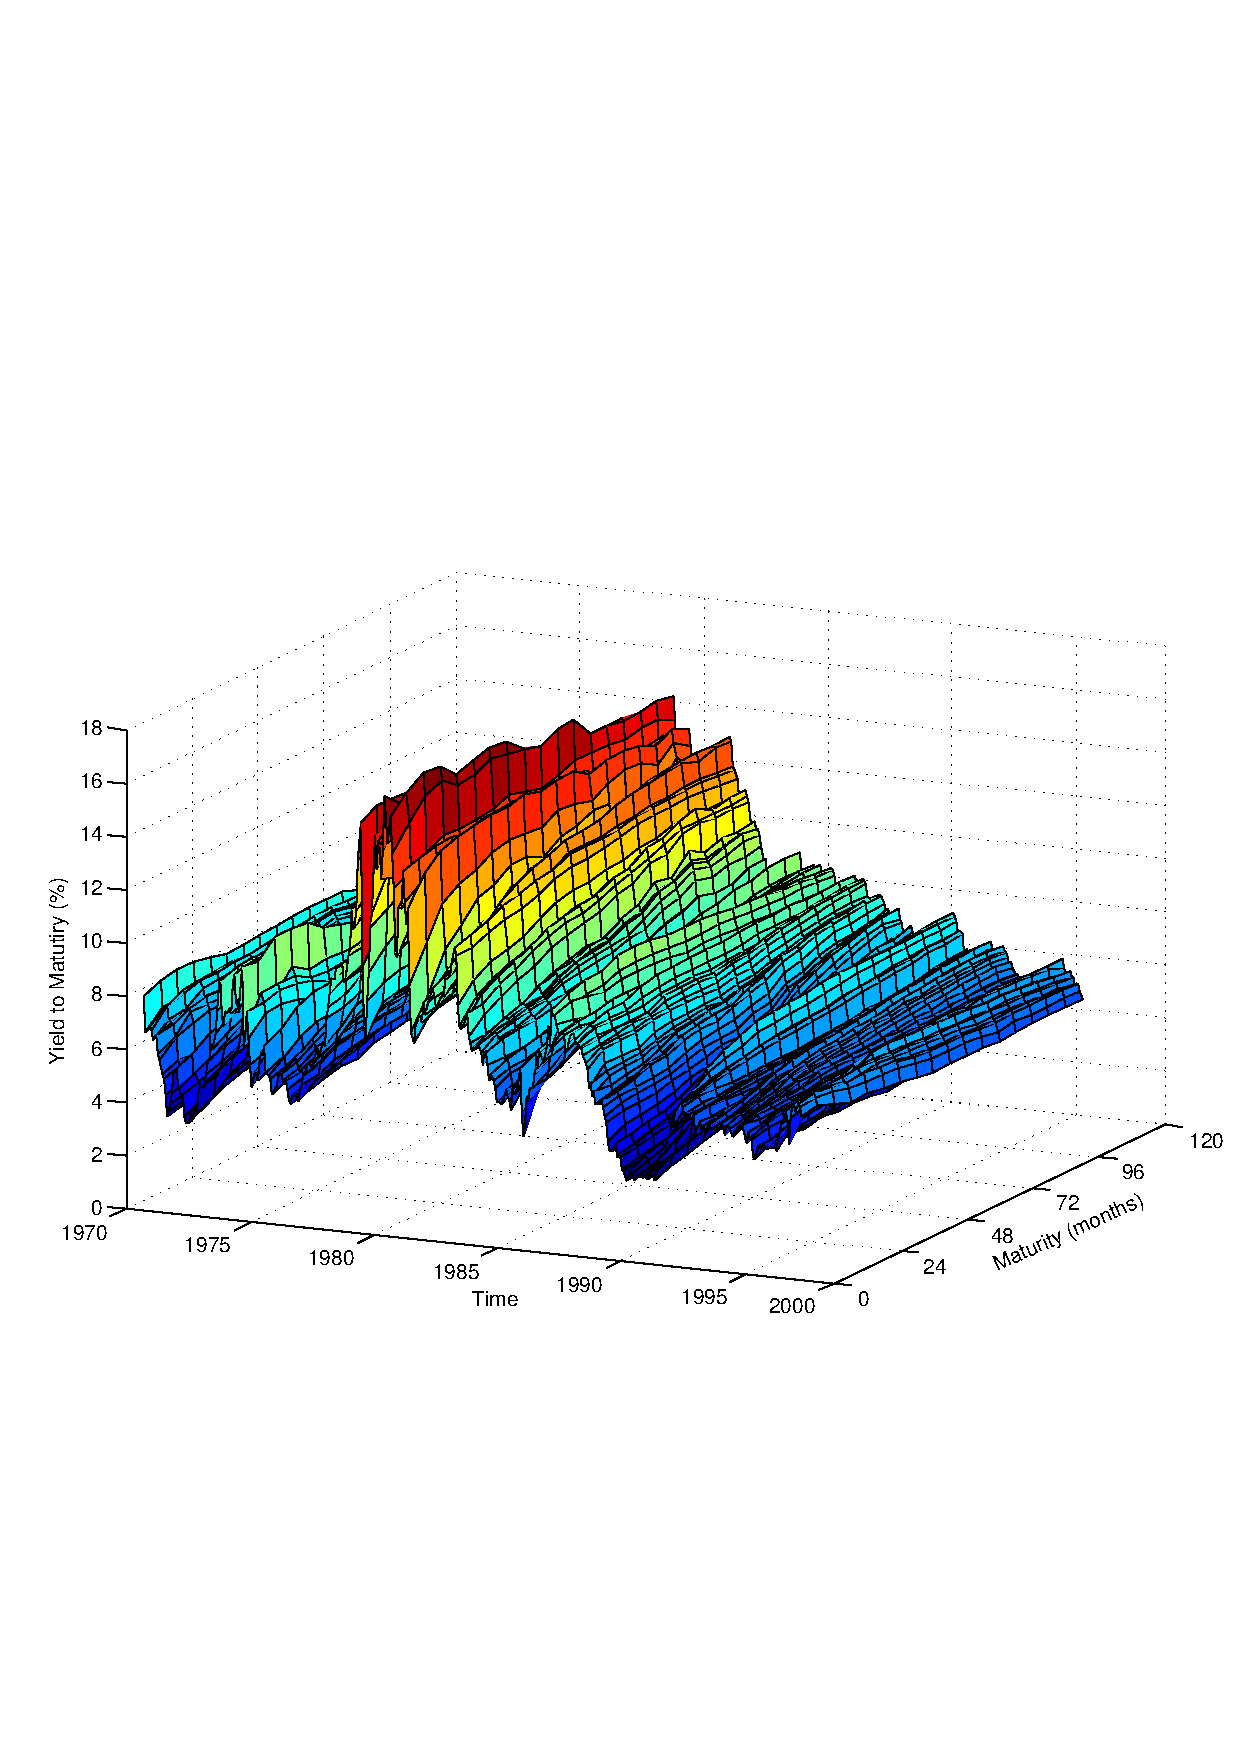
\includegraphics[width=15.5cm,height=11cm]{figures/tale_fig04}
   \caption{实际收益率曲线:1970:01--2000:12.}
   \label{tale_fig04}
  \end{figure}

图\eqref{tale_fig04}给出了整条收益率曲线的直观图形。表\eqref{summary_stat}则提供了样本数据的统计特征。关于收益率曲线的一些明显的特征化事实总结如下:
\begin{compactenum}[(i)]
  \item 一般而言,剩余到期期限越长,到期收益率越高,亦即长期收益率高于短期收益率。比如,期限为~1~个月的政府票据(bill)的收益率只有~6.4448,而~10~年期的国债券收益率则为~8.0474。总的说来,长短期国债券之间的利差关系变化体现在国债收益率曲线上,使国债收益率曲线表现出各不同的形态,在一定程度上预示了宏观经济发展周期的变化趋势。
  \item 水平因子呈现出较高的自相关关系,这说明长期收益率在比较稳定的范围内变动。在理论上,收益率曲线的两个主要特征——收益率差和收益率水平,两者都包含着整个市场未来的变化方向。收益率差反映了未来短期利率的变化,未来的短期利率包含着未来真实利率与市场对未来利率变化方向的理性预期。由于真实利率在长期中的波动是比较小的,未来短期利率的上升主要反映了市场的预期变化,在较长的预测时期尤其如此。
  \item 收益率曲线在短端的波动比长端的波动大。这也印证了水平因子的自相关系数较高,而斜度因子和曲度因子的自相关系数都比较低。收益率曲线的水平变化代表整体债券市场的未来变动方向。这个因子受到经济系统基础层面的影响,如代表性消费者的投资风险厌恶程度的改变、社会结构尤其是人口年龄结构的波动等。
\end{compactenum}

本文所使用的人口数据可以在美国人口调查局(BoC)的网站上查询到。这里,我采用\citeai{favero2012demographics}提供的已经整理的数据库\footnote{网页地址如下: \href{http://didattica.unibocconi.eu/myigier/index.php?IdUte=48917&idr=1753&lingua=eng}%
   {Prof. Carlo Favero's website}.}。在任何时点上,预测的~n~期~MY~比值是利用人口预测项目提供的有关数据计算的~n~ 期移动平均值。由于人口年龄结构具有比较稳定的变化趋势,通过计算出生率及死亡率,由社会色提供的人口模型能够为预测未来人口年龄结构变化提供相当准确的预测。当然,如\citeai{miles2012demographics}提到的,当重大的灾难性事件发生时,这一预测项目也可能不一定准确。然而,从市场理性预期的角度上看,这些关于未来的不确定风险已经包含在风险贴水中。因此,本文在使用人口数据时,已经预先的假定人口预测项目的可靠性。
   
%%%%%\clearpage  % 表格单独一页
\begin{center}\vspace{-1.5em}
  \vspace{-1.2em}
\begin{threeparttable} \centering
 \caption{收益率的描述性统计特征:1970:01--2000:12}
 \label{summary_stat}
 \renewcommand{\arraystretch}{1.1} \arrayrulewidth=0.6pt \tabcolsep=5.3pt
 \begin{tabular}{c c c c c c c c c}
   \hline \hline
  $\tau$ & Mean & Sd.Dev. & Mix & Max
   & $\hat{\rho}(1)$ & $\hat{\rho}(3)$ & $\hat{\rho}(12)$ & $\hat{\rho}(30)$ \\
   \hline \renewcommand{\arraystretch}{1.0} %%%% 
    1 &  6.4448 &  2.5824  & 2.6920 & 16.1620 &  0.9653  & 0.8943  & 0.6897  & 0.2797\\
    3 &  6.7549 &  2.6553  & 2.7320 & 16.0200 &  0.9720  & 0.9081  & 0.7113  & 0.2956\\
    6 &  6.9826 &  2.6619  & 2.8910 & 16.4810 &  0.9737  & 0.9104  & 0.7274  & 0.3321\\
    9 &  7.1047 &  2.6398  & 2.9840 & 16.3940 &  0.9736  & 0.9104  & 0.7343  & 0.3562\\
   12 &  7.2006 &  2.5693  & 3.1070 & 15.8220 &  0.9723  & 0.9080  & 0.7378  & 0.3744\\
   15 &  7.3057 &  2.5174  & 3.2880 & 16.0430 &  0.9741  & 0.9146  & 0.7464  & 0.3995\\
   18 &  7.3783 &  2.5022  & 3.4820 & 16.2290 &  0.9750  & 0.9168  & 0.7529  & 0.4183\\
   21 &  7.4412 &  2.4898  & 3.6380 & 16.1770 &  0.9760  & 0.9202  & 0.7564  & 0.4319\\
   24 &  7.4588 &  2.4428  & 3.7770 & 15.6500 &  0.9758  & 0.9179  & 0.7542  & 0.4412\\
   30 &  7.5517 &  2.3650  & 4.0430 & 15.3970 &  0.9755  & 0.9213  & 0.7640  & 0.4638\\
   36 &  7.6309 &  2.3408  & 4.2040 & 15.7650 &  0.9776  & 0.9274  & 0.7703  & 0.4767\\
   48 &  7.7687 &  2.2839  & 4.3080 & 15.8210 &  0.9782  & 0.9336  & 0.7755  & 0.4984\\
   60 &  7.8407 &  2.2483  & 4.3470 & 15.0050 &  0.9809  & 0.9382  & 0.7898  & 0.5179\\
   72 &  7.9566 &  2.2216  & 4.3840 & 14.9790 &  0.9811  & 0.9417  & 0.7987  & 0.5326\\
   84 &  7.9873 &  2.1819  & 4.3520 & 14.9750 &  0.9810  & 0.9393  & 0.7817  & 0.5351\\
   96 &  8.0460 &  2.1711  & 4.4330 & 14.9360 &  0.9827  & 0.9459  & 0.8063  & 0.5470\\
  108 &  8.0782 &  2.1796  & 4.4290 & 15.0180 &  0.9829  & 0.9465  & 0.8076  & 0.5523\\
  \midrule
120 ($\beta_1$)\tnote{1}
      &8.0474& 2.1353  & 4.4430 & 14.9250 &  0.9828  & 0.9447  & 0.7836  & 0.5433\\
$\beta_2$\tnote{2}
      &  1.2924 &  1.4246  &\hspace{-0.5ex}-3.5050 &  4.0600 &  0.9270  & 0.7855  & 0.4065  &\hspace{-0.5ex}-0.1188\\
$\beta_3$\tnote{3}
      &0.1152& 0.7073  &\hspace{-0.5ex}-1.8370 &  3.1690 &  0.7826  & 0.5586  & 0.2544  & 0.0746\\
   \hline \hline
 \end{tabular}
 %%
 \small{%
  \emph{注}:自相关系数为~95\%~置信区间。
 \begin{tablenotes}
\item [1] 实证的水平因子被定义为~10~年期到期收益率:$\beta_1=y(120)$;
\item [2] 斜度因子为:$\beta_2=y(120)-y(3)$;
\item [3] 曲度因子为:$\beta_3=2y(24)-y(120)-y(3)$。
\end{tablenotes}
}%
\end{threeparttable}
\end{center}
%\end{landscape}
%\restoregeometry
